\begin{frame}{Manipulación Atómica}
  \begin{columns}
    \begin{column}{0.4\textwidth}
      \begin{itemize}
        \item \textbf{Mecánica:} Arrastre lateral de átomos mediante fuerzas de Van der Waals.
        \item \textbf{Vertical:} Transferencia de átomos entre punta y superficie.
        \item \textbf{Propósito:} Construcción de estructuras personalizadas átomo por átomo.
        \item \textbf{Ejemplo:} El logo de IBM formado por 35 átomos de Xenón.
      \end{itemize}
    \end{column}
    \begin{column}{0.7\textwidth}
      \begin{figure}
        \centering
        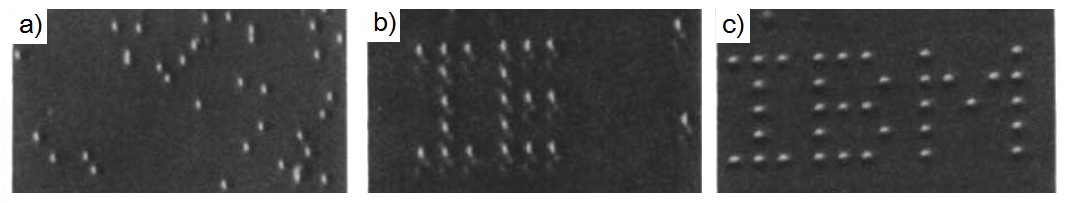
\includegraphics[width=\textwidth]{images/ejemplos/ibm_atoms.png}
        \caption{Manipulación de la punta de STM comenzando con a) muestra de xenón dosificada aleatoriamente, b) en construcción - mover el átomo de xenón a la posición deseada, y c) realización de la manipulación. }
      \end{figure}
    \end{column}
  \end{columns}
\end{frame}

% --- Corral Cuántico ---
\begin{frame}{Corrales Cuánticos}
  \begin{columns}
    \begin{column}{0.7\textwidth}
      \begin{figure}
        \centering
        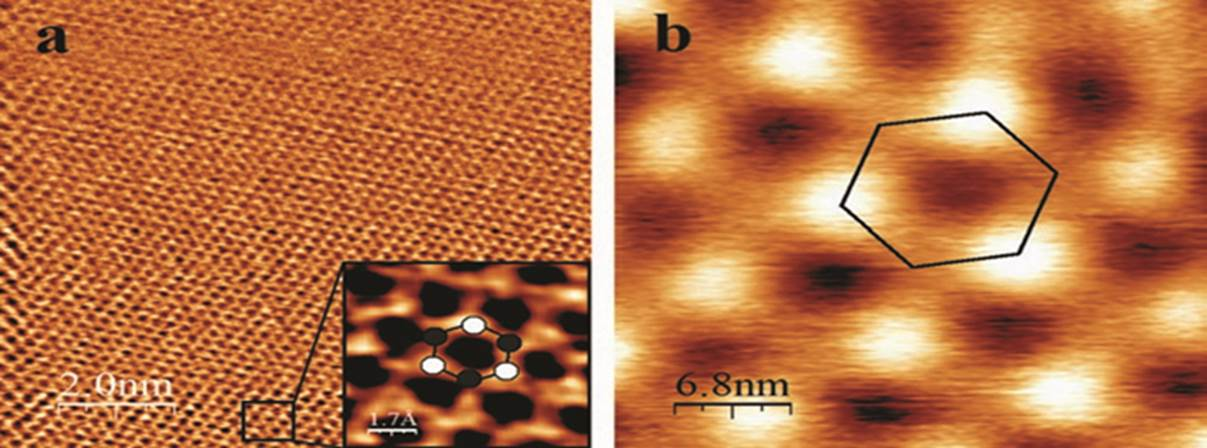
\includegraphics[width=\textwidth]{images/ejemplos/quantum_corral.png}
        \vspace{-0.8cm}
        \caption{Imágenes STM de HOPG: (a) Superficie normal con resolución atómica (0.246 nm entre puntos). Los puntos claros indican átomos de carbono sin un átomo en la capa inferior directa, mientras que los oscuros sí lo tienen. (b) Súperred que muestra un patrón hexagonal periódico, originado por un desajuste espacial entre la capa superficial y la inferior. Obtenidas con un equipo JEOL JSPM-5200 (resolución replicable con Nanosurf E-STM).}
      \end{figure}
    \end{column}
    \begin{column}{0.3\textwidth}
      \begin{itemize}
        \item \textbf{Confinamiento:} Barrera circular que atrapa electrones superficiales.
        \item \textbf{Interferencia:} Visualización de patrones de ondas estacionarias electrónicas.
        \item \textbf{Física:} Validación experimental de soluciones de la ecuación de Schrödinger en 2D.
      \end{itemize}
    \end{column}
  \end{columns}
\end{frame}

% --- Materiales 2D ---
\begin{frame}{Grafeno y Materiales 2D}
  \begin{itemize}
    \item \textbf{Red Hexagonal:} Confirmación de la estructura de panal de abeja del grafeno.
    \item \textbf{Patrones de Moiré:} Interferencia debida al desajuste de red entre capas.
    \item \textbf{Bordes:} Estudio de estados electrónicos en bordes tipo \textit{zigzag} y \textit{armchair}.
  \end{itemize}
  \begin{center}
    \begin{figure}
      \centering
      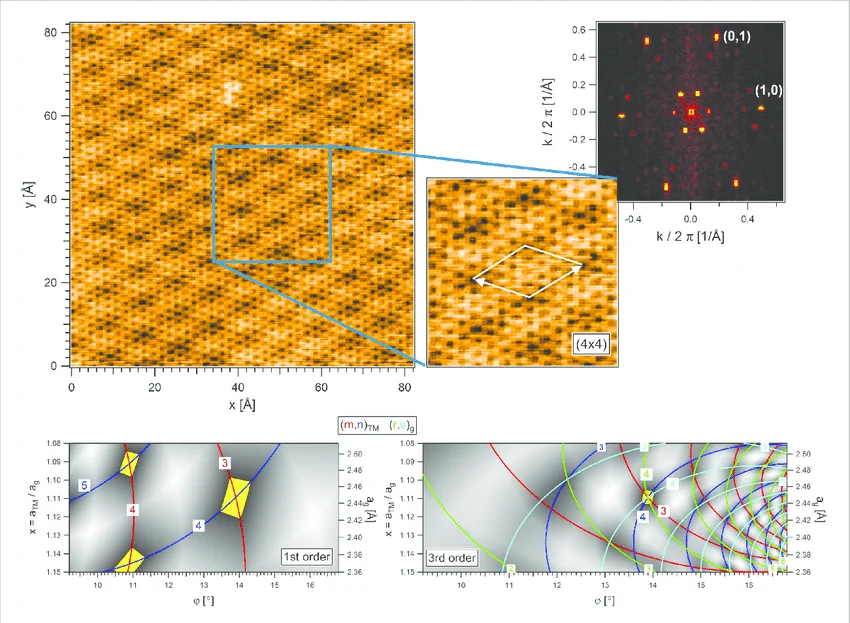
\includegraphics[width=0.5\textwidth]{images/ejemplos/graphene_moire.png}
      \vspace{-0.5cm}
      \caption{Estructura atómica y patrón de Moiré en grafeno.}
    \end{figure}
  \end{center}
\end{frame}

% --- Aplicaciones Biológicas ---
\begin{frame}{ADN y Biomoléculas}
  \begin{columns}
    \begin{column}{0.4\textwidth}
      \begin{itemize}
        \item \textbf{Estructura:} Resolución de la hélice de ADN y bases nitrogenadas.
        \item \textbf{Entorno:} Posibilidad de operar en medios líquidos para preservar muestras biológicas.
        \item \textbf{Autoensamblaje:} Estudio de monocapas autoensambladas (SAMs) de aminoácidos.
      \end{itemize}
    \end{column}
    \begin{column}{0.6\textwidth}
      \begin{figure}
        \centering
        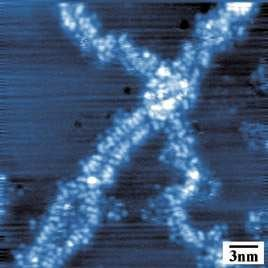
\includegraphics[width=0.8\textwidth]{images/ejemplos/dna_stm.png}
        \caption{Imagen STM de una molécula de ADN}
      \end{figure}
    \end{column}
  \end{columns}
\end{frame}

\begin{frame}{Validación Experimental: Teoría (DFT) vs. Experimento (STS)}

  % Texto explicativo corto en la parte superior
  \begin{itemize}
    \small
    \item \textbf{Aproximación de Tersoff-Hamann:} La Espectroscopía de Efecto Túnel (STS) mapea la Densidad Local de Estados (LDOS) de la muestra.
    \item La conductancia diferencial ($dI/dV$) es proporcional a la LDOS a una energía dada:
      $$ \frac{dI}{dV} \propto \rho_s(\vec{r}_0, E_F + eV) $$
  \end{itemize}
\end{frame}

\begin{frame}

  \begin{columns}
    % Columna Izquierda: Gráficas Teóricas (Apiladas verticalmente)
    \begin{column}{0.45\textwidth}
      \begin{figure}
        \centering
        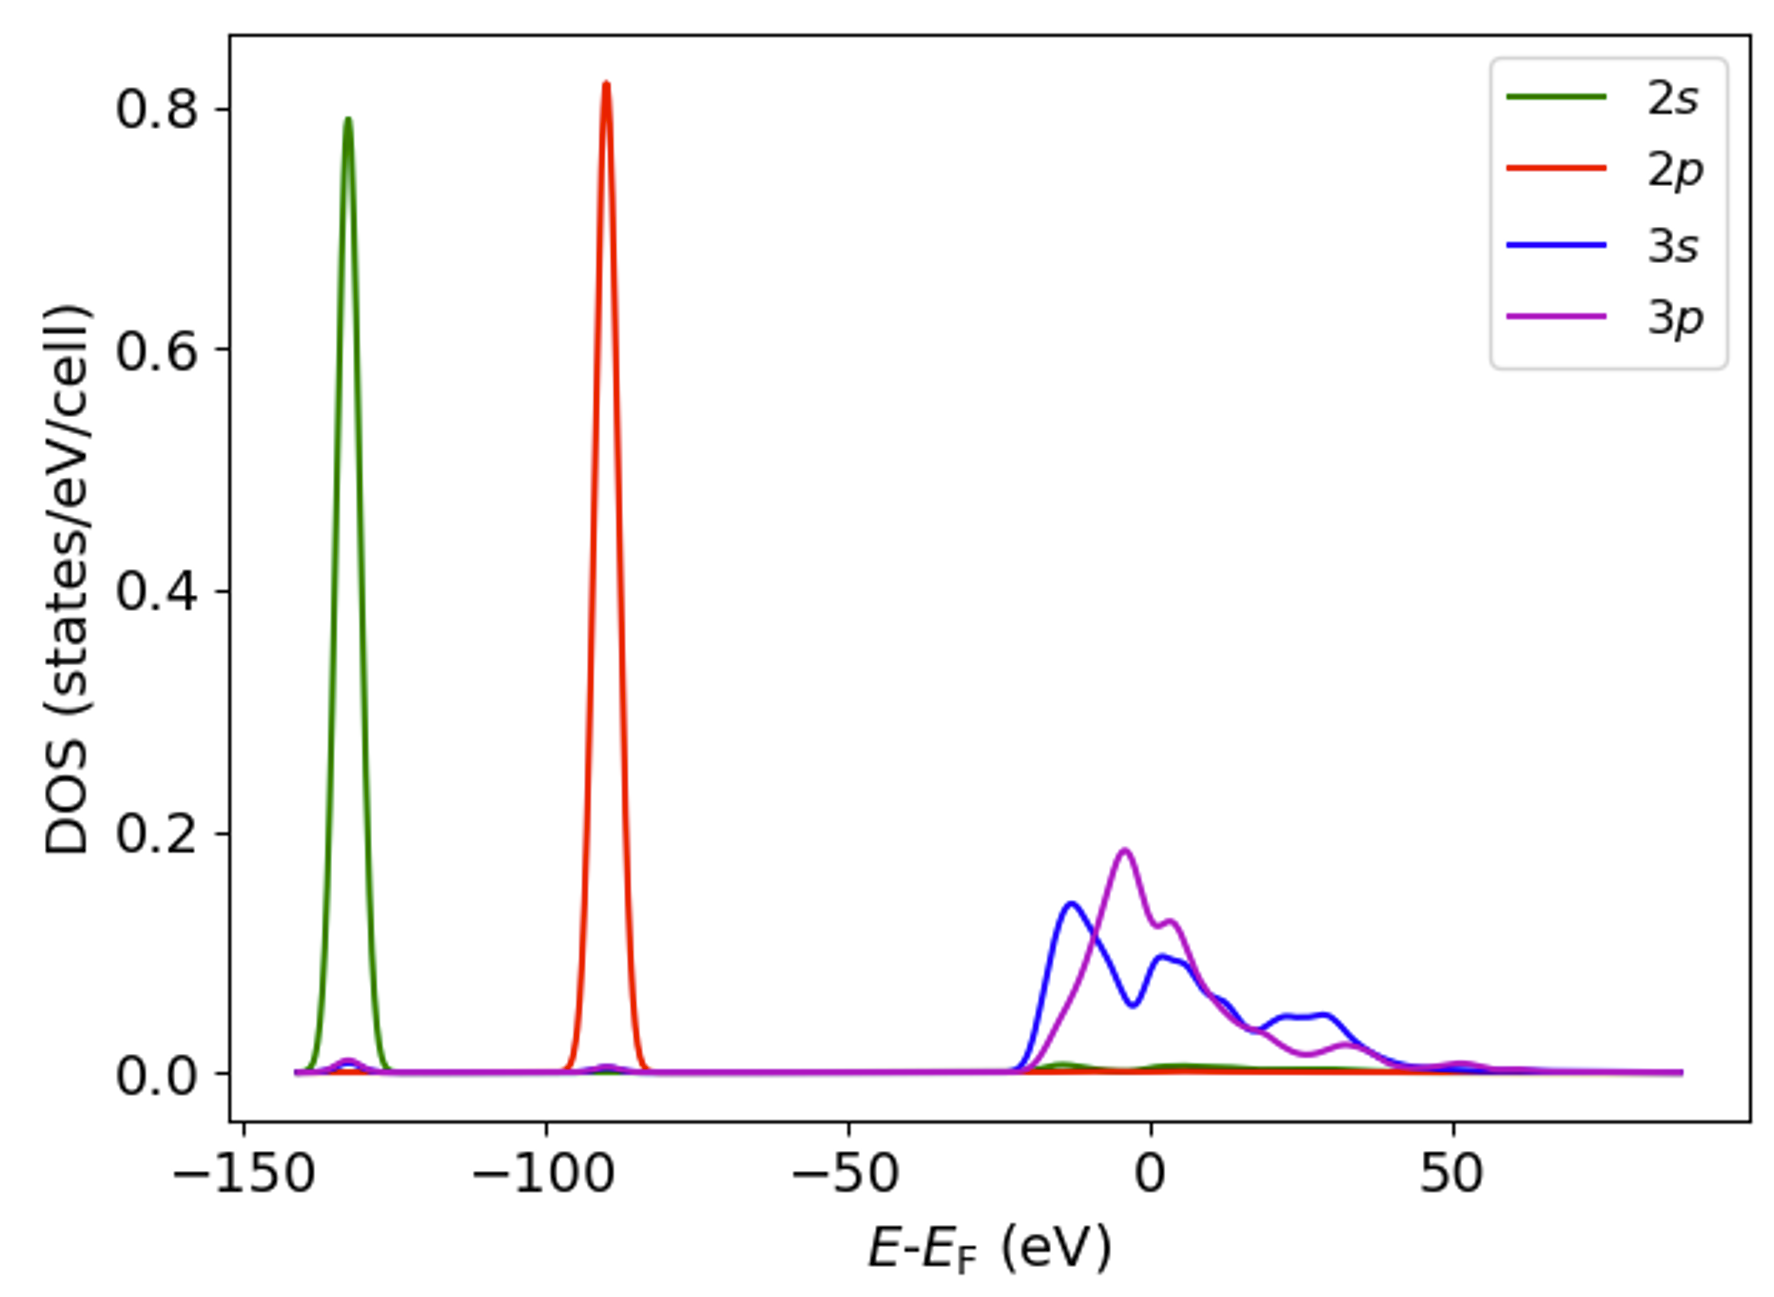
\includegraphics[height=0.3\textheight]{images/ejemplos/2SYQP.png}
        \caption{\scriptsize LDOS Teórica: Contribución espacial y de estados profundos.}
      \end{figure}
      \vspace{-0.6cm} % Ajuste vertical para acercar las gráficas
      \begin{figure}
        \centering
        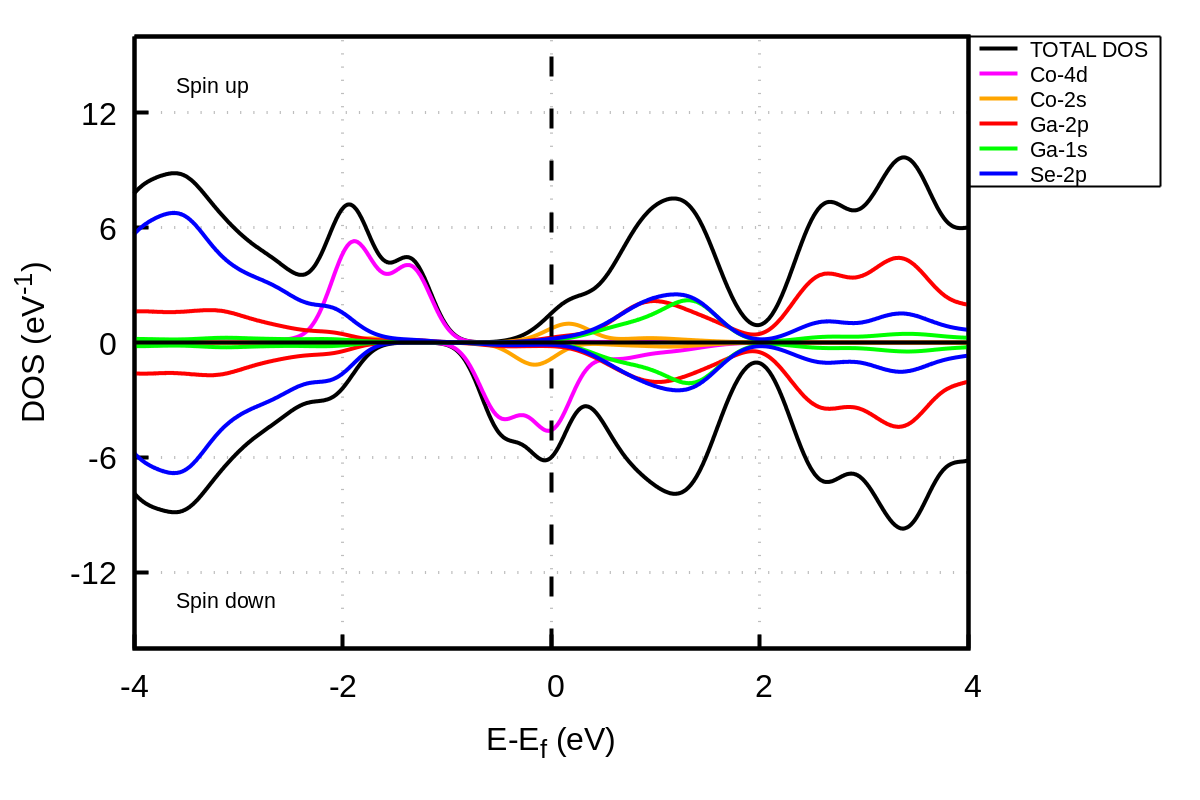
\includegraphics[height=0.3\textheight]{images/ejemplos/DOS-Co-GaSe-PSe.png}
        \caption{\scriptsize PDOS Teórico (QE): Proyección por orbitales.}
      \end{figure}
    \end{column}

    % Columna Derecha: Gráfica Experimental
    \begin{column}{0.5\textwidth}
      \begin{figure}
        \centering
        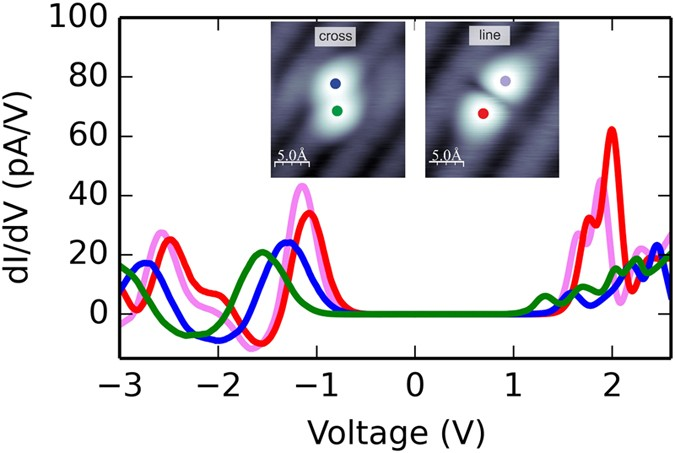
\includegraphics[width=\textwidth]{images/ejemplos/41598_2015_Article_BFsrep14496_Fig1_HTML.jpg}
        \caption{\scriptsize Conductancia diferencial experimental ($dI/dV$). Los picos se correlacionan con las bandas calculadas en DFT.}
      \end{figure}
    \end{column}
  \end{columns}
\end{frame}


% --- Tabla Comparativa ---
\begin{frame}{Comparativa de Técnicas}
  \begin{table}
    \centering
    \begin{tabular}{@{}llll@{}}
      \toprule
      \textbf{Característica} & \textbf{STM} & \textbf{AFM} & \textbf{SEM} \\ \midrule
      Mecanismo & Corriente túnel & Fuerza atómica & Haz electrones \\
      Resolución & Atómica ($<$0.1 nm) & Atómica ($\sim$0.1 nm) & 1-10 nm \\
      Muestra & Solo conductores & Conductores/Aislantes & Generalmente cond. \\
      Ambiente & Vacío/Aire/Líquido & Vacío/Aire/Líquido & Alto vacío \\ \bottomrule
    \end{tabular}
    \caption{Diferencias clave entre STM y otras microscopías de sonda/electrónicas.}
  \end{table}
\end{frame}
